%t PROJECT: <ETD> Electronic Thesis and Dissertation Initiative
%   TITLE: LaTeX report template for ETDs in LaTeX
%  AUTHOR: Neill Kipp, nkipp@vt.edu
%     URL: http://etd.vt.edu/latex/
% SAVE AS: etd.tex
% REVISED: September 6, 1997 [GMc 8/30/10]
% 

% Instructions: Remove the data from this document and replace it with your own,
% keeping the style and formatting information intact.  More instructions
% appear on the Web site listed above.

%\documentclass[12pt,dvips]{report}
\documentclass[12pt]{report}

\setlength{\textwidth}{6.5in}
\setlength{\textheight}{8.5in}
\setlength{\evensidemargin}{0in}
\setlength{\oddsidemargin}{0in}
\setlength{\topmargin}{0in}

\setlength{\parindent}{0pt}
\setlength{\parskip}{0.1in}

% Uncomment for double-spaced document.
% \renewcommand{\baselinestretch}{2}

% \usepackage{epsf}

% BHH Packages
\usepackage[]{mcode}
\usepackage[retainorgcmds]{IEEEtrantools}
\usepackage{amsmath}
\usepackage{amssymb}
\usepackage{graphicx,dblfloatfix}
\usepackage{subfig}
\usepackage{hyperref}
\graphicspath{ {./images/} }
\hypersetup{
    colorlinks=true,
    urlcolor=blue,
    citecolor=black,
    linkcolor=black
}
% END BHH Packages


\begin{document}

\newcommand{\fourier}{\mathcal{F}}

\thispagestyle{empty}
\pagenumbering{roman}
\begin{center}

% TITLE
{\large
Simulation of Various Channelizer Structures 
Directed by Cyclostationary Detector}

\vfill

Brian H. Hulette

\vfill

Project Report submitted to the Faculty of the \\
Virginia Polytechnic Institute and State University \\
in partial fulfillment of the requirements for the degree of

\vfill

Master of Engineering \\
in \\
Electrical Engineering

\vfill

Amir I. Zaghloul, Co-Chair \\
Jeffrey H. Reed, Co-Chair \\
T. Charles Clancy

\vfill

February 16, 2015 \\
Falls Church, Virginia

\vfill

Keywords: SDR, Cyclostationarity, Detection, Channelizer
\\
Copyright 2015, Brian H. Hulette

\end{center}

\pagebreak

\thispagestyle{empty}
\begin{center}

{\large Simulation of Various Channelizer Structures 
Directed by Cyclostationary Detector}

\vfill

Brian H. Hulette

\vfill

(ABSTRACT)

\vfill

\end{center}

One common problem in Software-Defined Radio (SDR) systems is the problem of
detecting and then isolating narrow signals of interest in wideband sampled
data. This involves using some means to detect the frequency of one or more
signals of interest and then tuning, filtering, and decimating them. This
problem is particularly challenging due to the high sample rate of this
wideband data, so efficient algorithms are very desirable. Solutions to this
problem have applications in many areas, including both Cognitive Radio and
Electronic Warfare.

A MATLAB simulation of an SDR framework for detecting and sub-band tuning
channelized signals is presented, with a focus on finding an efficient means to
combine the two algorithms. Detection is performed using the
spectral-correlation density function which exploits the cyclostationary
property of digital signals \cite{Gardner1}.  These detections are then used to
direct a channelizer which will tune, filter, and decimate all of the detected
signals. Two different channelizer structures are examined: a polyphase
analysis/synthesis channelizer \cite{Harris1} and an overlap-save filter bank
\cite{Borgerding1}.

A summary of relevant background information is provided.  This includes
a discussion of cyclostationarity and the spectral-correlation density function
as well as background on both channelizer structures. For the overlap-save
filter bank it will be shown that in many cases computation can be saved by
using the same FFT computation for both the cyclostationary detector and the
channelizer.

In this simulation, simple QPSK signals are used to model the signals of
interest, but the framework is applicable to any modulation or signal type that
has cyclostationary features. While other means of signal detection may be more
reliable for specific signals, a cyclostationary detector's primary strength is
its ability to function for many different types of digital signals.


\vfill

% GRANT INFORMATION

%That this work received support from the Southeastern Universities
%Research Association (SURA) ``Monticello Library Project'' is purely
%coincidental.

\pagebreak

% Dedication and Acknowledgments are both optional
% \chapter*{Dedication}
\chapter*{Acknowledgments}
First I must acknowledge the work of both Craig Carlson and Ruth Stoehr.
The core of my testbed for this project is a robust QPSK Transmitter/Receiver
pair we designed together for an ECE5654 project in the Spring of 2013.

I would like to thank my current employer, n~ask, inc., and all of my
co-workers there for their support, as well as  the .

I would also like to thank the members of my committee, particularly Dr.
Zaghloul, for their patience and support.

Finally, I would like to thank my friends and family, particularly my girlfriend
Meredith, for helping me through this years long process, and letting me use
``My Masters" as an excuse for nearly anything.

\tableofcontents
\pagebreak

\listoffigures
\pagebreak

%\listoftables
%\pagebreak

\pagenumbering{arabic}
\pagestyle{myheadings}

\chapter{Introduction}
\label{sec:intro}
\markright{Brian H. Hulette \hfill Chapter \ref{sec:intro}. Introduction \hfill}

A common problem when designing a Software-Defined Radio (SDR) system is the
problem of detecting and tuning signals of interest. A typical SDR will sample
at a relatively high rate to acquire a wideband signal. Then it will attempt to
detect the channels within the acquired frequency range that contain signals of
interest, and then tune, filter, decimate, and demodulate those signals. 

%TODO: links to SDR frameworks (webSDR) TODO: image of SDR plotting
Many popular SDR applications perform this detection step with
a ``man in the loop".  A falling raster of the wideband data is presented and
the man in the loop will select  the frequencies that he would like to process.
One common example of this is to acquire a wideband slice of the HAM radio
spectrum and then select different frequencies to demodulate new FM
Push-to-Talk signals and listen to them.

This paper investigates a structure that automates this process - but rather
than processing a single analog signal, this framework is intended to process
an arbitrary number of digital signals at once. Detection is performed by
a cyclostationary detector rather than by a man in the loop. This exploits the
cyclostationary properties exhibited by most digital signals with a fixed
symbol rate.  Tuning, filtering, and decimating is performed by a channelizer,
so that many signals can be processed at once.  Two different channelizer
structures are examined: a polyphase channelizer composed of an analysis
channelizer followed by several synthesis channelizer, and an overlap-save
filter bank. These structures are evaluated on two important criteria:
1) Their ability to accurately reproduce every detected signal, and 2) Their
computational efficiency when combined with a cyclostationary detector.
% TODO: list papers that discuss SCD for various protocols

Chapter~\ref{sec:cyclo} provides background information on cyclostationary
properties and the Specral Correlation Density (SCD) function upon which the
detector relies.  Chapter~\ref{sec:chan} discusses and compares both of the
channelizer structures that are simulated. Chapter~\ref{sec:sim}  discusses the
MATLAB simulation that was created and the results of it. Finally,
Appendix~\ref{sec:source} provides annotated source code for key parts of the
simulation, as well as locations where the entire source code can be found.

\chapter{Cyclostationary Detection}
\label{sec:cyclo}
\markright{Brian H. Hulette \hfill Chapter \ref{sec:cyclo}. Cyclostationary Detection \hfill}

\section{Cyclostationarity}
\label{sec:cyclo_prop}
Often signals are modeled as stochastic random processes with properties such as
mean and variance, but many man-made signals, particularly digital communications,
can be modeled with another statistical property called
\emph{cyclostationarity}, which implies the signal has some parameter which
varies with time. The frequency of this variation is called the cyclic
frequency, $\alpha$. \cite{Gardner1}.


Of particular interest for this project is second-order cyclostationarity,
where a signal has a periodic autocorrelation, R_{xx}(t, t+\tau):

\begin{IEEEeqnarray}{lCl}
    R_{xx}(t, t+\tau) = E\{x(t)x^*(t+\tau)\} = \sum_{\alpha} R_{xx}^{\alpha}(\tau)e^{j2 \pi \alpha t}
\end{IEEEeqnarray}

% TODO more detail here based on Oner1
The function $R_{xx}^{\alpha}(\tau)$ is the cyclic autocorrelation function (CAF), given by:

\begin{IEEEeqnarray}{lCl}
    R_{xx}^{\alpha}(\tau) = \lim_{T \to \infty} \frac{1}{T}\int_{-T/2}^{T/2} R_{xx}(t, t+\tau)e^{-j2\pi \alpha t} dt
\end{IEEEeqnarray}
The CAF is a function of two parameters, the cyclic frequency, $\alpha$ and the
delay, $\tau$. This function can be used for signal detection in the time
domain. An estimate of the function versus $\alpha$ and $\tau$ is computed,
then features within this plane can be used for detection.
% TODO: reference papers that perform time domain detection (listed in "Energy Efficient Spectrum Sensing using Cyclostationarity")
% "Cyclostationary Based Air Interface Recognition For Software Radio Systems" is also a time domain approach
However, what is of interest for this project is detection in the frequency
domain. This can be performed using the fourier transform of the CAF, called
the Spectral Correlation Density (SCD), giveb by:

\begin{IEEEeqnarray}{lCl}
    S_{xx}(\alpha, f) = \int_{-\infty}^{\infty} R_{xx}^{\alpha}(\tau)e^{-j2\pi f \tau} d\tau
\end{IEEEeqnarray}

The SCD is a generalization of the conventional Power-Spectral Density (PSD),
which it reduces to at $\alpha=0$ \cite{Oner1}. Like the CAF, the SCD also
contains unique features based on the modulation type, symbol rate, and carrier
frequency of the transmitted signal, which we can exploit for signal detection.
In \cite{Gardner2}, Gardner defines this SCD for various basic modulation
types, including QPSK, which is used in the presented simulation.

%\section{Exploiting Cyclostationarity for Detection}
%\label{sec:exploit_cyc}
%For the problem defined in Chapter \ref{sec:intro} we can define the wideband
%signal $W(t)$ as the sum of $N$ cyclostationary signals, tuned to
%various frequencies, in an AWGN channel:
%\begin{IEEEeqnarray*}{lCl}
%    W(t) & = & \sum C_{i}(t) e^{j 2 \pi f_i t} + N(t)
%\end{IEEEeqnarray}
%
%Where the $C_i(t)$ are cyclostationary random processes at various symbol rates,
%tuned to corresponding frequencies $f_i$ and $N(t)$ is the AWGN.

%
%We would like to exploit the cyclostationarity of the $C_i$ waveforms to
%identify the frequency, $f_i$, of those waveforms which are transmitted at a
%specific symbol rate.

\section{Estimating the SCD}
\label{sec:estimating_scd}
% Use Gardner1 to show that SCD is conjugate multiplication of frequency shifted spectra
% TODO:
% - cyclic wiener relation on Gardner1 pg. 153
% - attempts to derive in lab notebook pg. 20-21
% or just cite Gardner1?
We can compute a slice of the SCD at cyclic freqency $\alpha$ as
the cross spectral density of the two frequency-shifted time sequences
$x_L(t) = x(t)e^{j\pi\alpha t}$ and $x_U(t) = x(t)e^{-j\pi\alpha t}$.

\begin{IEEEeqnarray}{lCl}
    S_{xx}(\alpha, f) & = & X_L(f)X_U^* (f)
\end{IEEEeqnarray}

Note that $x_L(t)$ has been shifted down in frequency by $\alpha/2$, and
$x_U(t)$ has been shifted up by the same amount. In order to estimate the SCD
in this way we must perform two FFTs: one for both $X_L(f)$ and $X_U(f)$.
However, it is possible to estimate both of these spectra using a single FFT,
$X(f)$, in some cases:

\begin{IEEEeqnarray}{lCl}
    S_{xx}(\alpha, f) & = & X_L(f)X_U^* (f) \\
                      & = & X(f - \alpha/2)X^*(f + \alpha/2)
\end{IEEEeqnarray}

Usign the second relation we can compute $S_{xx}(\alpha, f)$ using a single
forward FFT by shifting that FFT in either direction by $\alpha/2$, and
then conjugate multiplying the two shifted spectra together. This is
significant, since a simple forward FFT of the acquired data is useful for
other operations, such as channelization, as we will see in Section
\ref{sec:os_filter_bank}.

Of course there is a caveat. In order to perform this shift accurately using a
single FFT we need to circular shift the FFT by an integer number of bins.  This
means we can only accurately perform this frequency shift when $\alpha/2$ is
a multiple of the FFT resolution.  Thus $\alpha$ must satisfy the following
relationship:
\begin{IEEEeqnarray}{lCl}
    \alpha = \frac{2kf_s}{N_{fft}} \text{, } k \in \mathbb{Z}
\end{IEEEeqnarray}

If an estimate of the SCD at a cyclic frequency that does not satisfy this
relation is required, then we must take the original approach (perform the
frequency shift in the time domain) to be perfectly accurate. Alternatively, we
can still use a single forward FFT and approximate the shift by interpolating
between bins, but this is only an approximation.


\chapter{Channelizer Structures}
\label{sec:chan}
\markright{Brian H. Hulette \hfill Chapter \ref{sec:chan}. Channelizer Structures\hfill}
\section{Polyphase Analysis/Synthesis Channelizer}
\label{sec:poly_chan}
Fred Harris has described the related structures that he calls Polyphase
Analysis and Polyphase Synthesis Channelizers \cite{Harris1}. A Polyphase
Analysis channelizer can be used to break up a wideband signal into $D$ distinct
channels, each decimated by a factor of $D$ from the wideband sample rate. The
channelized frequencies are integer multiples of the output sample rate:

\begin{IEEEeqnarray}{lCl}
    f_k = k \frac{f_s}{D}
\end{IEEEeqnarray}

where $f_k$ is the center frequency of channel $k$ and $f_s$ is the input sample
rate. A Polyphase Synthesis Channelizer performs the reverse operation - it
combines $D$ distinct channels with equal sample rate into a single wideband
signal.

These two structures can be combined to create a very flexible channelizer that
can tune channels with arbitrary center frequencies and various bandwidths
\cite{Harris2} - a simplified version of this structure is discussed in
Section~\ref{sec:combine_analysis_synthesis}.

In \cite{Harris1}, Harris shows how the Polyphase Analysis Channelizer works by
starting with a basic filter/decimator and making incremental modifications
until it becomes an Analysis Channelizer as shown in Figure
\ref{fig:polyphase_analysis}. A brief summary of this description is provided here, which follows Figure~\ref{fig:polyphase_proof}.

\begin{figure}[h!]
\centerline{
    \subfloat[Single channel of a simple tuning, filtering, and decimating channelizer. $h(n)$ is a baseband low-pass filter.]
    {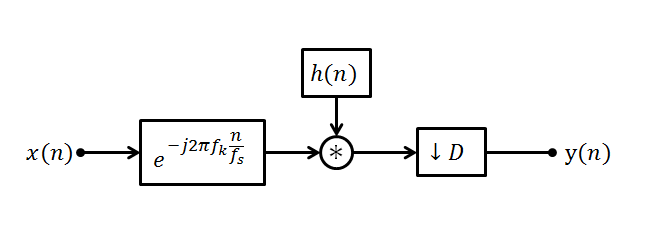
\includegraphics[width=0.45\textwidth]{polyphase_1}%
    \label{fig:polyphase_1}}
    \hfill
    \subfloat[Equivalency theorem allows the tuning step to be moved after the decimation. The baseband filter must be shifted up to $f_k$. If $f_k$ is a multiple of the output sample rate,  $\frac{f_s}{D}$, the tuning step can be dropped.]
    {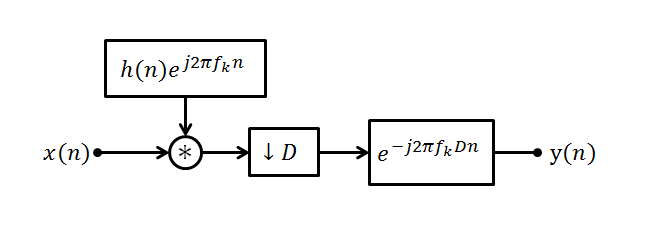
\includegraphics[width=0.45\textwidth]{polyphase_2}%
    \label{fig:polyphase_2}}
}
\centerline{
    \subfloat[The Noble Identity allows the filtering and decimation to be combined to remove excess computations.]
    {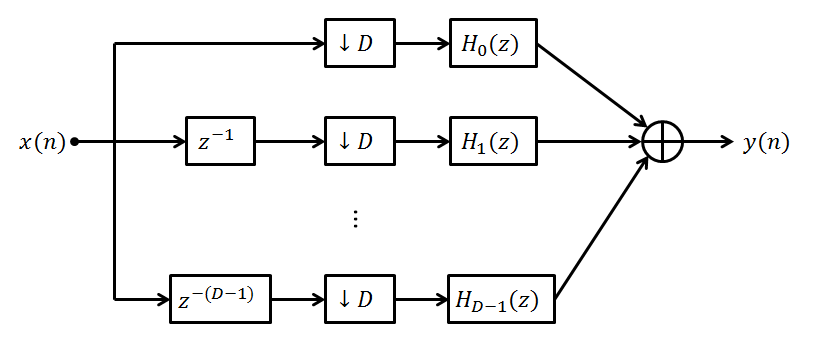
\includegraphics[width=0.45\textwidth]{polyphase_3}%
    \label{fig:polyphase_3}}
    \hfill
    \subfloat[The series of delays and decimation steps can be replaced with an input commutator and complex phasors can be added after each filter to select channel $k$.]
    {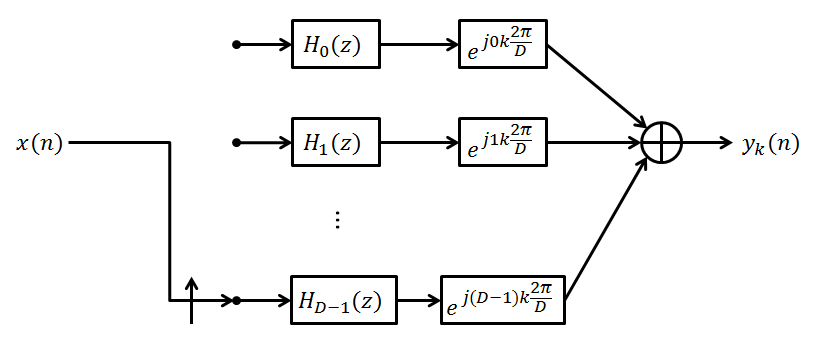
\includegraphics[width=0.45\textwidth]{polyphase_4}%
    \label{fig:polyphase_4}}
}
\caption{Creating a single channel of a polyphase analysis channelizer}
\label{fig:polyphase_proof}
\end{figure}

We start with a single channel of a very basic channelizer in Figure
\ref{fig:polyphase_1}. This channel consists of a multiplication with a complex
phasor to tune the desired center frequency down to baseband, followed by
a low-pass filter, represented by $h(n)$, and finally a decimation by $D$. The
first modification we can make takes advantage of the Equivalency Theorem,
which says that we can switch the order of the tuner and the filter, \textbf{if}
the filter is changed to a bandpass filter centered at $f_k$. This modification
is shown in Figure \ref{fig:polyphase_2}. In this figure the tuner has also
been moved after the decimator. Note that if the channel frequency, $f_k$, is
an integer multiple of the output sample rate, $\frac{f_s}{D}$, then the tuner
simplifies to $e^{j2\pi n} = 1$, so it can be dropped completely.  Thus we will
restrict the polyphase analysis channelizer to center frequencies which are
integer multiples of the output sample rate.

Next we can use the Noble Identity to switch the place of the decimation and
the filter, as shown in Figure \ref{fig:polyphase_3}. In order to do so we need to define a set of new filters, $H_r(z)$, such that:

\begin{IEEEeqnarray}{lCl}
    H(z) = H_0(z^D) + z^{-1}H_1(z^D) + \hdots + z^{-(D-1)}H_{D-1}(z^D)
\end{IEEEeqnarray}

This means that each filter, $H_r(z)$, has has an impulse response which is $h(n)$
shifted by $r$ samples and decimated by $D$. Using the Noble Identity in this
way saves us from performing computations for samples that will just be dropped
by the decimator. Note that in Figure \ref{fig:polyphase_3} the tuner has been
dropped since we are restricting the channelizer to frequencies which are
multiples of the output sample rate.

Finally, we complete the structure for a single channel of a polyphase analysis
channelizer in Figure \ref{fig:polyphase_4}. The combination of delays and
decimators at the front of the previous structure is actually just
a commutator. In \cite{Harris1} Harris explains this by thinking about the
decimators as a switch that closes every $D$ samples. So in Figure
\ref{fig:polyphase_3}, when all of the switches close the filter at the bottom
gets the oldest sample, and each filter as you go up gets one newer sample
until you get to the most recent sample on the top. The next sample is not
processed until the switches close again, and it is passed to the filter at the
bottom. With this explanation it is easy to see the whole structure can be
replaced with a commutator.

The final structure has one more modification. The outputs are multiplied by complex phasors which select the individual channel, $k$, centered at $f_k$. For more info on why this works refer to \cite{Harris1}. The great thing about these complex phasors is that the set of phasors that are multiplied and then summed together for channel $k$ correspond to the $k$th output of a DFT:

\begin{IEEEeqnarray}{lCl}
    y_k(n) & = & \sum_{r=0}^{D-1} y_r(n) e^{j(2\pi/D)rk} 
\end{IEEEeqnarray}

Where $y_r(n)$ represents the output of filter $H_r(z)$, and $y_k(n)$ is the
output of channel $k$. Thus we can compute all $D$ of the complex phasors with
a D-point FFT, as shown in Figure \ref{fig:polyphase_analysis}. Figure
\ref{fig:polyphase_synthesis} shows the complementary structure: the Polyphase
Synthesis Channelizer. It is essentially a mirror image of the Analysis case
- an IFFT followed by filters and a reverse commutator. It combines $D$
channels at an equal sample rate, $f_s$, into a single wideband signal at
sample rate $Df_s$. The following section shows how these two structures can be
used together to produce a very flexible channelizer.

% TODO: reverse commutator? is that a thing?

\begin{figure}[h!]
\centerline{
    \subfloat[Analysis]
    {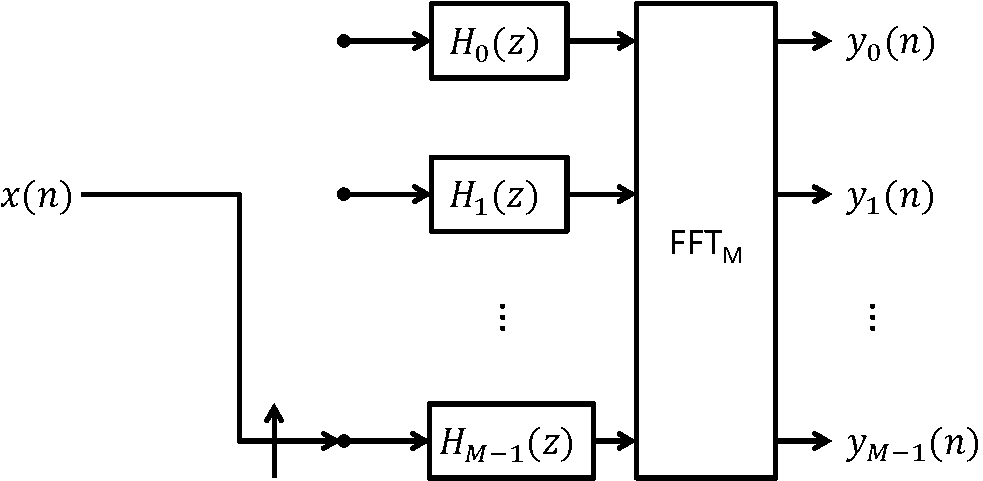
\includegraphics[height=4cm]{polyphase_analysis}%
    \label{fig:polyphase_analysis}}
    \hfill
    \subfloat[Synthesis]
    {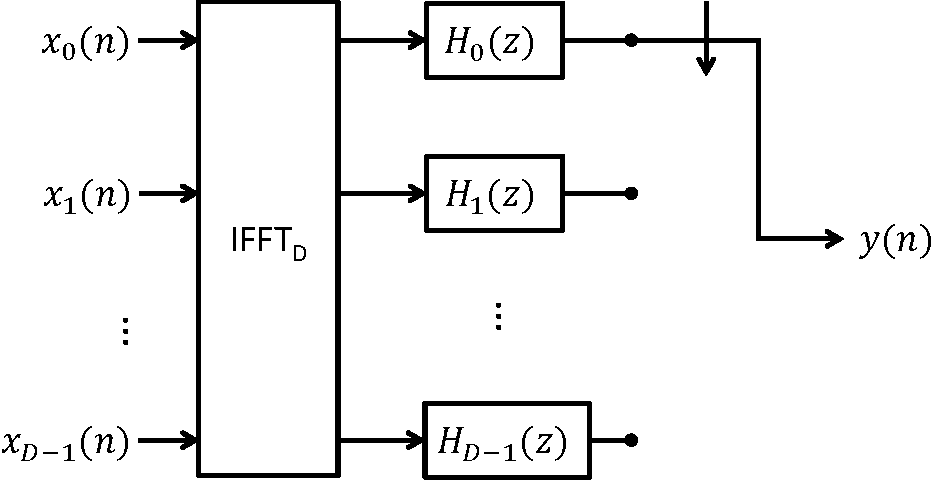
\includegraphics[height=4cm]{polyphase_synthesis}%
    \label{fig:polyphase_synthesis}}
}
\caption{Full Polyphase Analysis/Synthesis Channelizer Structures}
\label{fig:poly_analysis_synthesis_structs}
\end{figure}

\subsection{Combining Analysis and Synthesis Channelizers}
\label{sec:combine_analysis_synthesis}
The primary limitations of an Analysis Channelizer alone are that 1) it is limited
to a single output sample rate, and 2) the channel center frequencies must be
a multiple of that output sample rate. This is perfectly acceptable when every
signal being processed is at the same bandwidth and symbol rate, and they are
channelized with a known spacing, but in many SDR applications this is not the
case. One solution to this problem is to use analysis and synthesis structures
\emph{together} to create one very flexible strucuture.

Figure \ref{fig:analysis_and_synthesis} illustrates one simple way that this
might be implemented. The first step of this process uses an Analysis
Channelizer to break up the wideband into small equal parts (1). Then,
Synthesis Channelizers are used to re-combine the parts of the signal that
correspond to signals of interest (2). Finally, complex phasors are used to
remove the frequency offset created by the Synthesis Channelizers, as well as
any residual offset based on the desired center frequency (3).

\begin{figure}[h!]
    \begin{center}
    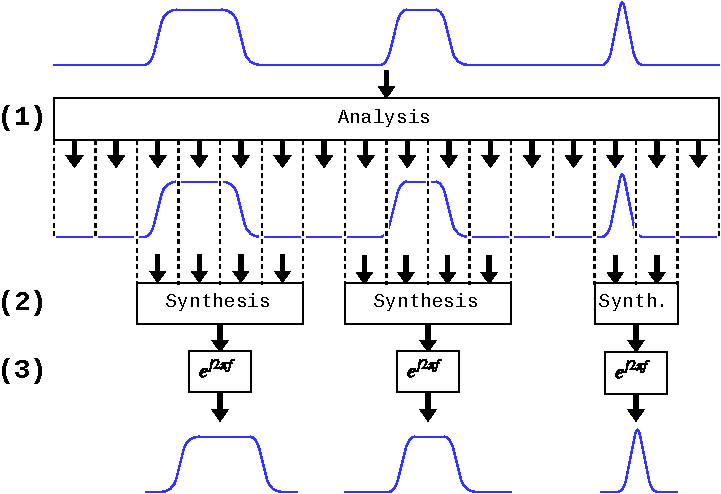
\includegraphics[width=0.8\textwidth]{polyphase}%
    \end{center}
    \caption{
Using Polyphase Analysis/Synthesis Channelizer Structures in concert. Step (1)
is an Analysis Channelizer that breaks the signal into 16 channels, Step (2) is
a set of Synthesis Channelizers for each signal of interest, and Step (3) is
a complex phasor that corrects the frequency offset. Note that this figure
depicts the signal in the frequency domain, simply for ease of illustration -
all inputs and outputs are time-domain signals.
    }
    \label{fig:analysis_and_synthesis}
\end{figure}

The analysis channelizer can be running all the time, while the synthesis
channelizers and phasors in steps (2) and (3) can be dynamically allocated as
signals of interest are detected (by some external detector).

\cite{Harris2} describes a more complex take on this same concept, but this
simplified version is sufficient for this project.
% TODO: more detail about Harris2 if I want to bring it up



\subsection{Limitations}
\label{sec:poly_limitations}
This structure has a couple of obvious limitations if a Polyphase Analysis
Channelizer is used by itself. Every channel must be at the same output sample
rate, $f_s/D$, and they must have center frequencies which are multiples of
that sample rate.

If the combination analysis/synthesis structure is used then this limitation
can be avoided, however there are still limitations. First, the output sample
rate must still be a decimation of the input sample rate - arbitrary rates are
not allowed. Second, while the output signals can be reconstructed quite well
after they have been split by the analysis channelizer, the reconstruction is
not perfect and could introduce errors. Harris discusses the concept of
a ``perfect reconstruction" filter \cite{Harris2} which may cirumvent this
limitation, but it is beyond the scope of this project.

Finally, there is no obvious way that this structure can be efficiently
combined with SCD estimation for detection. Nothing about an analysis
channelizer can be re-used for the detection approach used in this project.

% TODO analysis of computational complexiy for polyphase vs cyclo

\subsection{Advantages}
\label{sec:poly_advantages}
The primary advantage of a lone Polyphase Analysis Channelizer is its simplicity and efficiency, but its limitations make it an untenable solution for this project.

The combination Polyphase Analysis/Synthesis Channelizer adds a significant
amount of complexity, but it is still quite efficient for the amount of
flexibility that it provides.

% TODO: more stuff

\section{Overlap-save Filter Bank}
\label{sec:os_filter_bank}
The ``overlap-save filter bank" structure used in this simulation is based
entirely on a description by Mark Borgerding from March 2006
\cite{Borgerding1}.  Borgerding's concept is based on the well known
Overlap-Save fast convolution technique.

% TODO cite Borgerdings [1]-[5] here for Overlap-Save?
OS fast convolution can be used to speed up convolution with
a filter that has a long impulse response. The concept is that rather than
convolving in the time-domain, $O(N^2)$, it is faster to first
perform an FFT of both the signal and the filter and multiply in the frequency
domain, then IFFT to go back to the time domain, $O(N\log_2N)$.
There is nothing new about this idea, but Borgerding's innovation is that he
shows how to extend this concept to tune, filter and decimate any number of
channels with arbitrary frequencies and bandwidths.

This report uses the same terms that Borgerding defines:

\begin{tabular}{ll}
    $x(n)$        & Input data \\
    $h(n)$        & Baseband filter response \\
    $y(n)$        & Tuned, filtered and decimated output data \\
    $P$           & Length of $h(n)$ \\
    $N$           & FFT size \\
    $D$           & Decimation factor \\
    $V = N/(P-1)$ & Ratio of FFT size to filter order \\
\end{tabular}

\begin{figure}[h!]
\centerline{
    \subfloat[Performing frequency shift by circular shifting the FFT output]
    {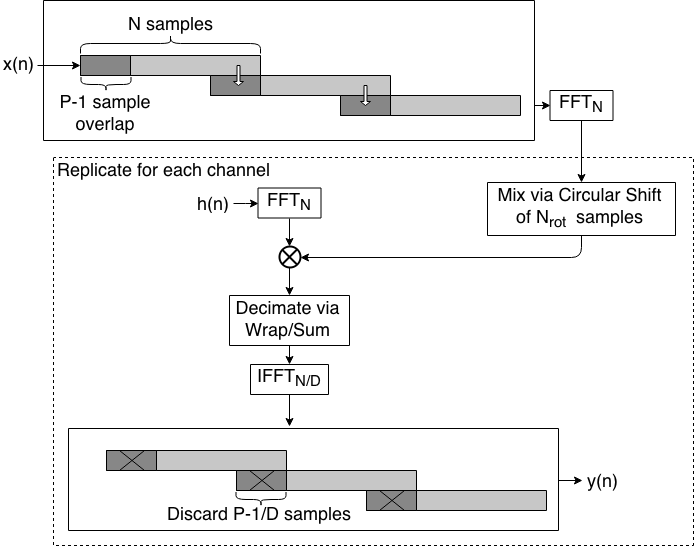
\includegraphics[width=0.45\textwidth]{overlap_save_shift}%
    \label{fig:overlap_save_shift}}
    \hfill
    \subfloat[Performing precise frequency shift in the time-domain]
    {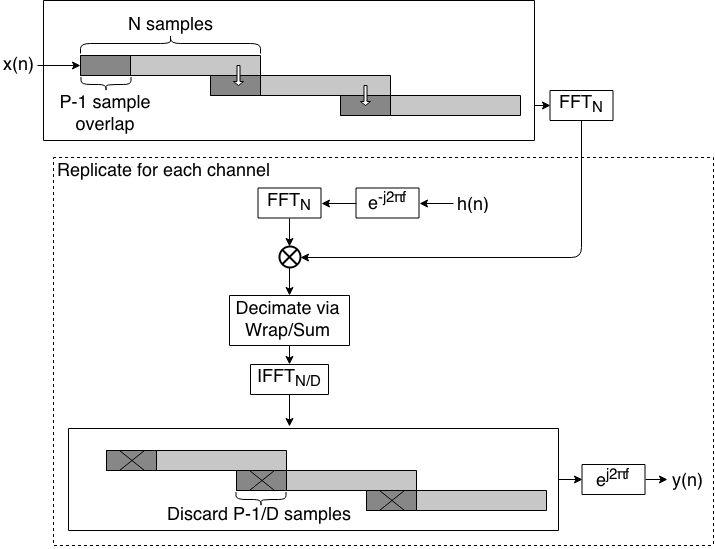
\includegraphics[width=0.45\textwidth]{overlap_save_time_domain}%
    \label{fig:overlap_save_time_domain}}
}
\caption{Overlap-Save Filter Bank Structures}
\label{fig:overlap_save_filter_banks}
\end{figure}

\emph{Tuning:} If the frequency of the signal of interest corresponds to one of
the FFT bins then we can simply circular shift the FFT output to place that bin
at the center. Then filtering can be performed at baseband.  If all channels
satisfy this criteria then we can re-use a single forward FFT for every
channel, simply by circular shifting it to the appropriate bin in every case. 
This approach is shown in Figure \ref{fig:overlap_save_shift}

However, if this condition is not satisfied then we will need to perform the
frequency shift in the time domain by multiplying by a complex phasor.
Fortunately, there is a still a way to re-use the forward FFT in this case.
After taking an FFT of the non frequency-shifted signal we can shift the
baseband filter response up to the desired frequency, then after the filtered
signal is IFFT'd back into the time domain, we perform the frequency shift with
a complex phasor.  This is even better than frequency shifting before the
forward FFT since the multiplication is performed after decimation. This
approach is shown in Figure \ref{fig:overlap_save_time_domain}.

\emph{Decimation:} Following the frequency domain filtering we have two
different options for decimation. The first option is to perform a full size
inverse FFT of the output, and then decimate in the time domain. The issue with
this approach is that we are computing a larger inverse FFT than we really need
to. As a solution to this, Borgerding suggests decimating in the frequency
domain. The approach (called ``Wrap/Sum" in Figure
\ref{fig:overlap_save_filter_banks}) is simple: coherently add together the aliased
components of the frequency spectrum.  For example, if the FFT size is 1024 and
we need to decimate by a factor of 4, then coherently sum FFT samples 0 to 255,
256 to 511, 512 to 767 and 768 to 1024.  The result is a 256 sample frequency
spectrum which we can now inverse FFT to produce the decimated output. The only
trick with this approach is that we must discard just $(P-1)/D$ samples rather
than $P-1$ to accont for the overlap.  This reveals one restriction of this
structure: the filter order $P-1$ must be an integer multiple of the
decimation, $D$.

\subsection{Limitations}
\label{sec:os_limitations}
There are a few limitations of this structure that are worth mentioning. First,
as mentioned earlier, the filter order $P-1$ must be an integer multiple of the
decimation factor $D$. This problem is pretty easy to solve though, simply
zero-pad the filter to achieve an appropriate length. Another limitation that
is potentially challenging is that the FFT size, $N$, must be an integer
multiple of the decimation rate, $D$. So decimation rates whose prime factors
are larger than 2 or 5 (or others, depending on the FFT implementation) could
lead to FFT inefficency for this structure.

One more limitation occurs when attempting to rotate the FFT to frequency
shift.  As previously mentioned, the precision of the frequency shift is
limited by the resolution of the FFT. However, the precision is also limited
further by $V$, the ratio of ,FFT size to filter order. This is because we must
restrict mixing to the frequencies whose period completes in $L=N-(P-1)$
samples. Borgerding provides the following equation for computing the number of
FFT bins to rotate to shift to frequency $f$ (\cite{Borgerding1} Equation (1)):

\begin{equation*}
    N_{rot} = \text{round}\left( \frac{Nf}{Vf_s} \right) V
\end{equation*}

Where $f_s$ is the base sample rate. This equation simply adjusts $N_{rot}$ to
the nearest multiple of $V$ bins. It is worth noting that my solution for
making $P-1$ an integer multiple of $D$ is only making this problem worse by
making $V$ larger - but there's nothing to be done about that other than opting
for a shorter filter.

\subsection{Advantages}
\label{sec:os_advantages}

The greatest benefit of the Overlap-Save Filter Bank for my application is
the ease with which it can be combined with SCD Estimation for cyclostationary
detection. Obviously, the first step for both algorithms is a forward FFT of the
wideband input. If we were to design a joint cyclostationary
detector/Overlap-Save Filter Bank we could re-use the same forward FFT for both
algorithms.

The only design challenge (which is certainly significant) is finding
a combination of FFT size, sample rate, and decimation factor that will work
for both algorithms.

% TODO: Analysis of this problem. Decimation factor is related to alpha by the amount of oversampling.
% Started this analysis a bit in lab notebook pg. 23

%We can say that the output sample rate is some integer multiple of the symbol rate:
%\begin{equation}
%    f_s' = \beta \alpha \text{, } \beta = 1,2,\hdots
%\end{equation}
%Where the integer multiple $\beta$ is simply the amount of oversampling. Then we can 

Additionally, averaging the overlapped FFT frames together may have an effect
on the accuracy of the SCD estimation, but analyzing this effect is beyond the
scope of this project.

\chapter{Simulation}
\label{sec:sim}
\markright{Brian H. Hulette \hfill Chapter \ref{sec:sim}. Simulation \hfill}
A MATLAB simulation of these structures has been written. Directions to find
all of the source code can be found in Appendix \ref{sec:source}. Each module
- testbench, cyclostationary detector, polyphase analysis channelizer, and
overlap-save filter bank - was developed and tested separately. The detector
was then combined with each channelizer and their performance was evaluated.
The same logical flow is followed in this Chapter as the modules are presented.

\section{Testbench}
Each Module is tested with the same wideband signal. A waveform sampled at 10 MHz with three QPSK signals:
\begin{itemize}
    \item{312.5 ksymbols/s at -2.5 MHz}
    \item{156.25 ksymbols/s at 0 MHz}
    \item{625 ksymbols/s at 2.5 MHz}
\end{itemize}
Note that the symbol rates were all chosen as fractions of the wideband sample
rate by design, as this allows the approximation discussed in
Section~\ref{sec:estimating_scd} to be used.

\begin{figure}[h]
    \begin{center}
        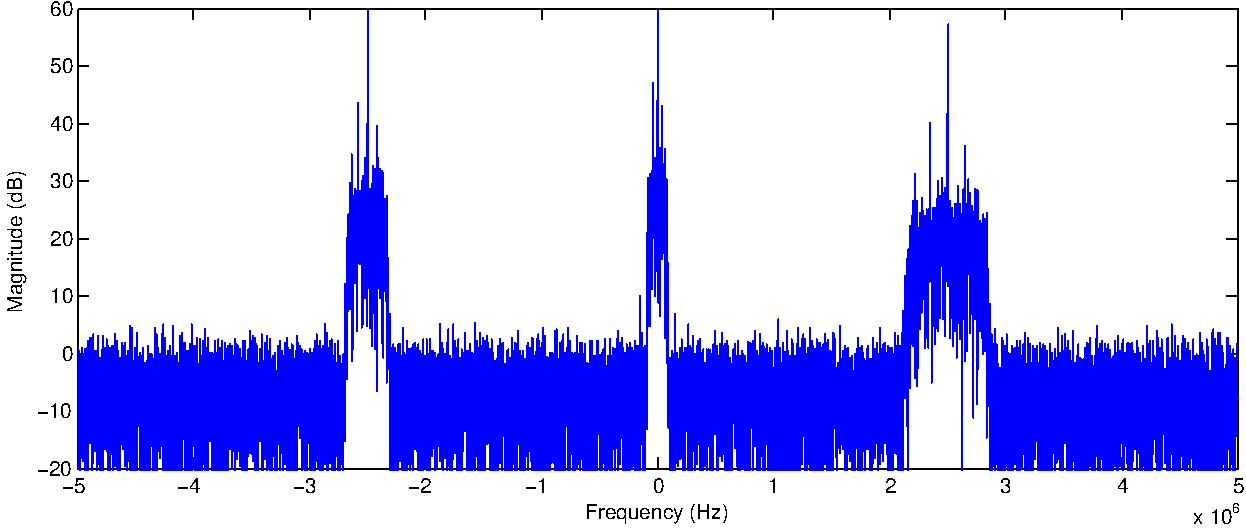
\includegraphics[width=0.95\textwidth]{test_signal}
    \end{center}
    \caption{Test signal used for each module}
\end{figure}

A simulation of a QPSK transmitter/receiver pair is used to generate the
signals used in this signal, and to attempt to demodulate the output of the
channelizers. This trasmitter channel encodes the data with a convolutional
code, packetizes the encoded data, and appends a synchronization sequence to
each packet. The receiver uses a squared spectrum to correct any major
frequency offsets, then uses the synchronization sequence to correct timing and
phase offsets. on a per packet basis. Finally, it performs channel decoding and
outputs the demodulated bits. More detail can be found in the project report, available at
\url{https://github.com/TheNeuralBit/cyclo_channelizer/raw/master/reference/ECE5654_Project_Report.pdf}.

\section{Cyclostationary Detector}
\label{sec:sim_cyclo}
The first module is the cyclostationary detector. The detector works by
computing estimates of the SCD at particular cyclic frequencies and searching
for features. The first step, estimating the SCD, can be performed by the
MATLAB function \texttt{cyclic\_spectrum(...)}, which will compute an estimate
of the given data at a specific cyclic frequency, $\alpha$.  It accepts a few
additional parameters:

\begin{description}
    \item[Mode:] Set to either of the techniques described in Section
    \ref{sec:estimating_scd}: Exact time-domain frequency shifts, or a single
    FFT with frequency-domain shifts. The latter is what we are primarily concerned
    with, for its efficiency.
    \item[FFT Size:] Size of the FFT used to go to the frequency domain.
    \item[Averaging:] Will average N estimates together to produce a more accurate
    result.
\end{description}

According to \cite{Gardner2}, QPSK signals generate a large peak in the SCD at
the signal's center frequency when $\alpha$ is equal to the signal baud rate.
So for this application estimates are generated at cyclic frequencies
corresponding to baud rates of interest. Figure \ref{fig:cyclo_estimates} shows
examples of these estimates for our test signal.

\begin{figure}[bh!]
\centerline{
    \subfloat[SCD at $\alpha = 0$, Equivalent to a PSD]
    {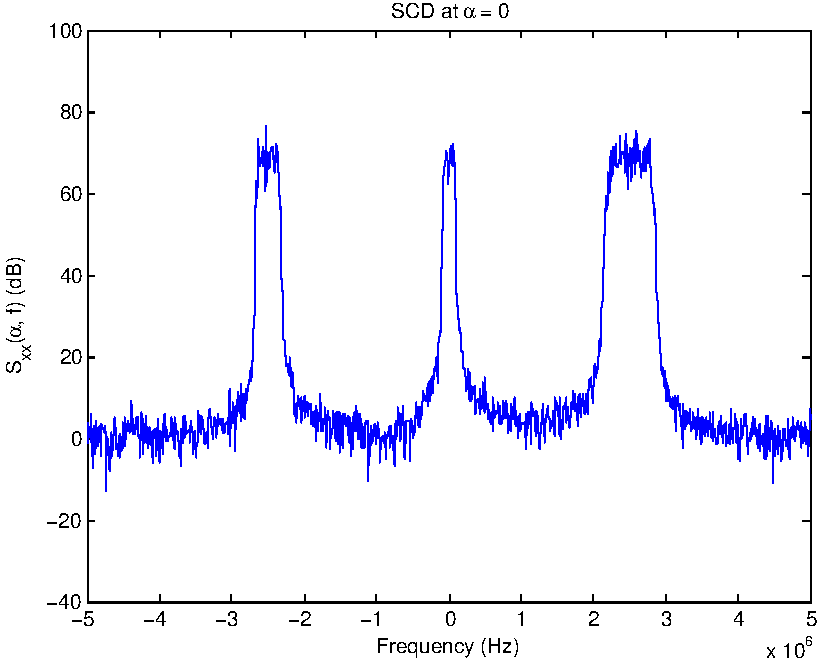
\includegraphics[width=0.45\textwidth]{cyclo_0}%
    \label{fig:cyclo_0}}
    \hfill
    \subfloat[SCD at $\alpha = 156.25$ kHz]
    {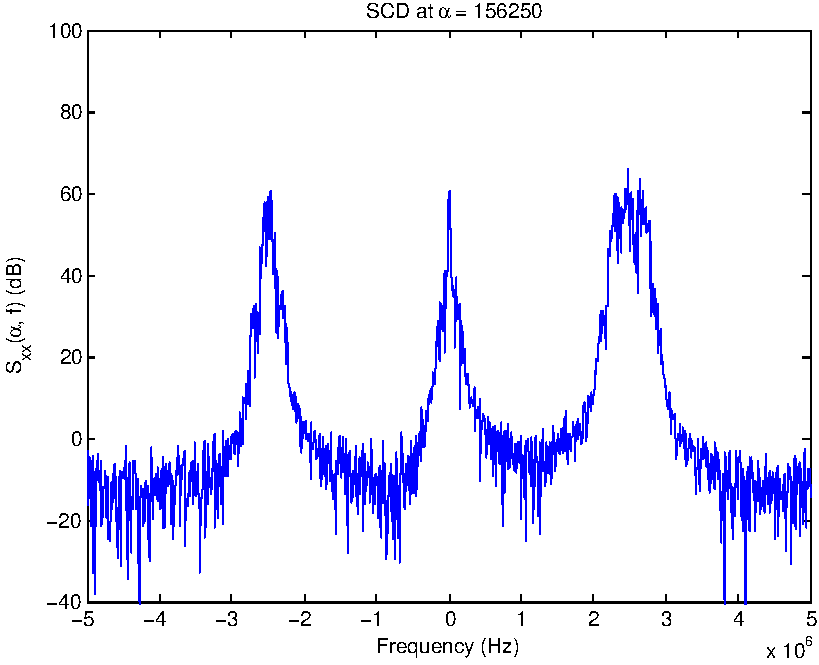
\includegraphics[width=0.45\textwidth]{cyclo_156250}%
    \label{fig:cyclo_156250}}
}
\centerline{
    \subfloat[SCD at $\alpha = 312.5$ kHz]
    {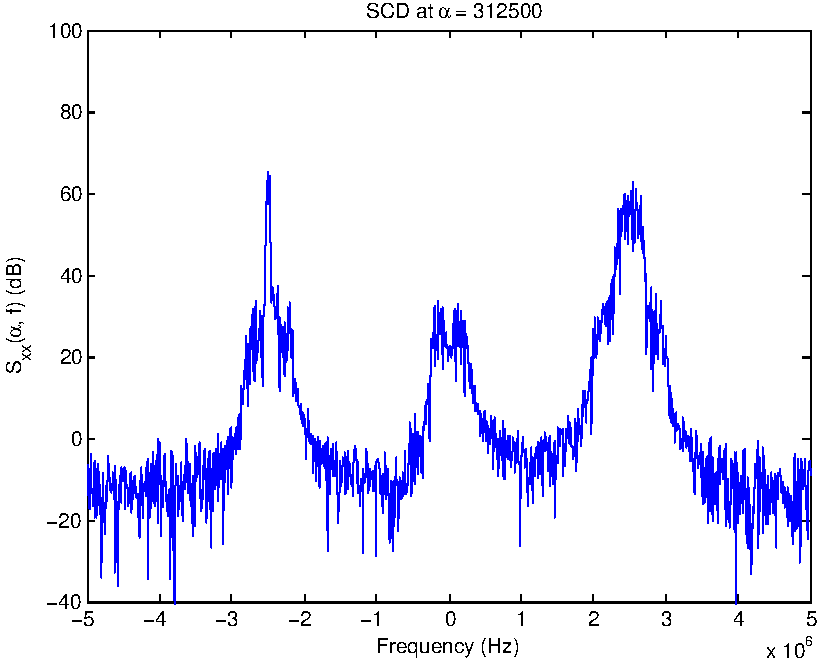
\includegraphics[width=0.45\textwidth]{cyclo_312500}%
    \label{fig:cyclo_312500}}
    \hfill
    \subfloat[SCD at $\alpha = 625$ kHz]
    {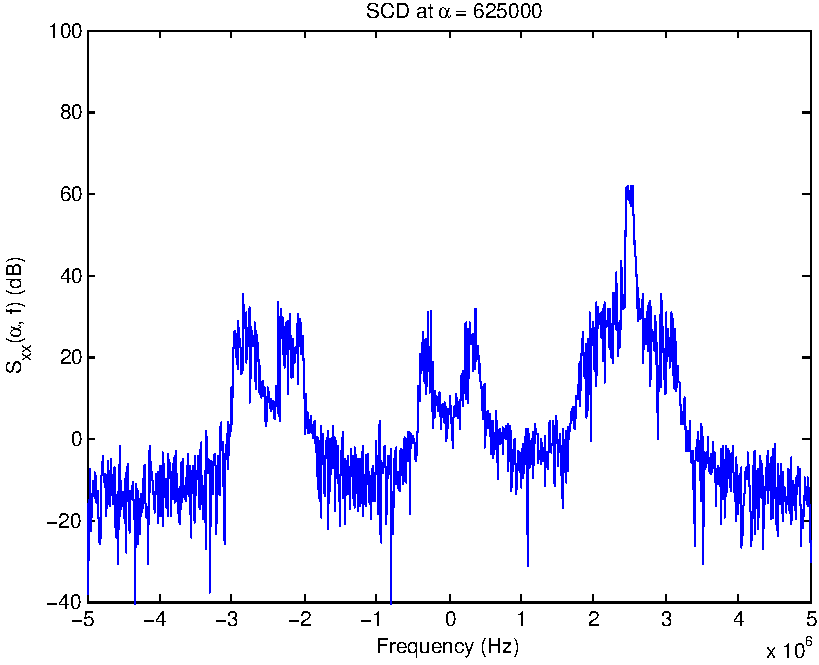
\includegraphics[width=0.45\textwidth]{cyclo_625000}%
    \label{fig:cyclo_625000}}
}
\caption{Estimates of the SCD at various cyclic frequencies. FFT size = 1024, Averaged over 10 FFTs.}
\label{fig:cyclo_estimates}
\end{figure}

In each of these estimates it easy to detect the large, narrow peak at the
center frequency of the signal with the corresponding baud rate. However, there
are also other features, which agree with the theoretical SCD from
\cite{Gardner2}.  The higher baud rate signals generate wide peaks in the lower
cyclic frequency estimates, like the peak at 2.5 MHz in Figure
\ref{fig:cyclo_156250}. These are easy to distinguish from the main peak with
the human eye (less easily with a computer), since they are much wider. The
lower baud rate signals also generate features in the higher cyclic frequency
estimates, in the form of two, much smaller peaks, straddling the actual center
frequency. Examples of this are visible at 0 MHz in Figure
\ref{fig:cyclo_312500} and \ref{fig:cyclo_625000}. These features are easily
filtered out by either a human or a computer with a simple threshold.

The second portion of the cyclo detection must use these SCD estimates to 
generate a list of detected frequencies, and the corresponding signal's
baud rate. In order to do so the following algorithm has been devised. It accepts the input wideband data, and a list of potential baud rates that are of interest.

\begin{enumerate}
    \item Initialize two empty lists \texttt{f[]} (center frequencies) and \texttt{b[]} (corresponding baud rate for each frequency)
    \item Sort list of potential baud rates from lowest to highest
    \item Estimate SCD at $\alpha$ equal to the first (lowest) baud rate
    \label{loop_ref}
    \item Detect peaks in the SCD. Use a threshold and a minimum peak separation
        to filter out false alarms.
    \item For each detected peak, check if an entry already exists in
        \texttt{f[]} near that frequency. If so, replace it with this peak's
        frequency and replace the corresponding entry in \texttt{b[]} with
        $\alpha$. Otherwise, append a new entry to \texttt{f[]} and
        \texttt{b[]} with the same values.
    \item Repeat from \ref{loop_ref} using the next baud rate in the list
\end{enumerate}

This is a very simple algorithm, but it works well for this test. It is
fully implemented in the \texttt{cyclo\_detect(...)} function. In an actual
application a more robust approach should be used. One possibility which could
be investigated but is beyond the scope of this project would be to use
a morphological filter to isolate only very narrow peaks. Between that and the
thresholding, other features would be easily ignored. For this project the
simple approach was taken, because the primary focus is on efficiently
estimating the SCD.

There is a major limitation to the implementation of this approach which is
important to note.  The SCD estimates are generated only based on the beginning
of the input signal. This means that signals are detected based on only the
first $N_{FFT}N_{Avg}$ samples. This works well in this application
since the test signals are on at the beginning of time and continue until there
is no more data to transmit, but in reality signals are going up and down
all the time. In an actual application the cyclostationary detector should be
run continuously to detect new signals as soon as they come up, and to detect
when they go away.

\section{Polyphase Analysis Channelizer}
\label{sec:sim_poly}
The simulation of the polyphase analysis channelizer is broken up into three
major parts: \texttt{analysis\_channelizer(...)},
\texttt{synthesis\_channelizer(...)}, and \texttt{polyphase\_channelizer(...)}.  The
latter of these combines the first two to implement the flexible channelizer
described in Section~\ref{sec:combine_analysis_synthesis}.

The implementation of \texttt{analysis\_channelizer(...)} accepts time domain
input data and a number of channels to produce, and outputs that number of
channels in the time domain. No additional configuration is necessary.
A low-pass filter with cut-off at the output's nyquist frequency is designed and
used. The output is indexed such that the first channel above $-f_s/2$ is in
index 1, the chanel at baseband is in index $D/2$, and the channel at $f_s/2$
is in index $D$.  This indexing is illustrated in
Figure~\ref{fig:polyphase_channel_indexing}.

% TODO create this figure

\texttt{synthesis\_channelizer(...)} is designed to perfectly complement
\texttt{analysis\_channelizer(...)}, so it will accept the list of channelized
data produced by the synthesis channelizer, and it will produce a replica of
the original input. Internally, it designs and uses a low-pass filter with
cutoff at the input's nyquist frequency. Note that this means an analysis
channelzier immediately followed by a synthesis channelizer of the same size
will use the same filter internally.

% TODO: mention that assumption is even number of channels

Finally, \texttt{polyphase\_channelizer(...)} utilizes both of these functions to
implement a flexible channelizer structure.  It accepts the input data its
sample rate and two additional confiuration parameters:
\begin{description}
    \item[Frequencies:] A list of the center frequencies of the signals of interest
    \item[Decimations:] A list of the decimation factors to be used for each
        corresponding center frequency.  Every decimation factor must be
        a factor of the highest decimation factor.
    result.
\end{description}
The simulation will first create a synthesis channelizer with decimation equal
to the highest requested decimation (Step (1) from
Figure~\ref{fig:analysis_and_synthesis}), Figure~\ref{fig:polyphase_splits}.  For
all requested outputs with this decimation factor, the nearest output of the
analysis channelizer will be frequency shifted so that the desired center
frequency is at baseband, and passed through. For every remaining output,
a synthesis channelizer will be produced to combine the channels surrounding
that frequency (Step (2)) and a complex phasor will shift the desired center
frequency down to baseband (Step (3)).

\begin{figure}[bh!]
    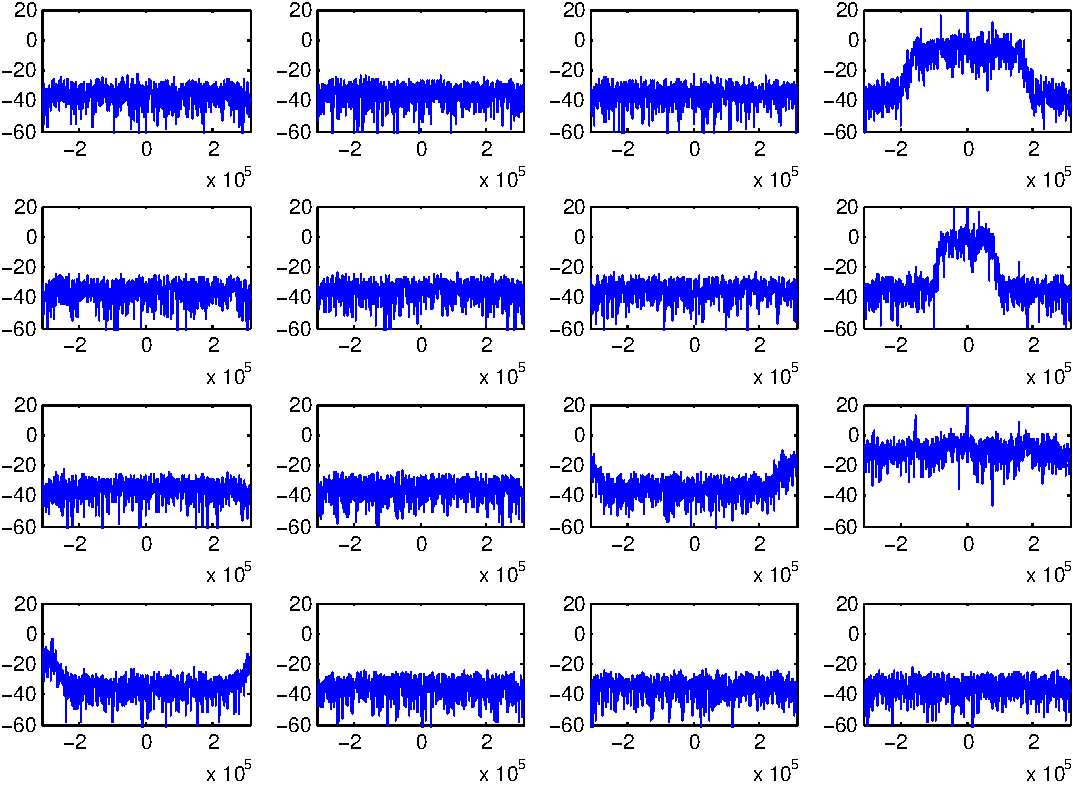
\includegraphics[width=\textwidth]{polyphase_splits}%
    \caption{Output of a 16 channel polyphase analysis channelizer operating on
             the test signal. X Axes are frequency in Hz, Y Axes are magnitude
             in dB}
    \label{fig:polyphase_splits}
\end{figure}

The major limitation of this implementation is that certain frequencies
at the highest decimation factor \emph{cannot} be produced. Any signal at the
boundary between two outputs of the analysis channelizer will not be
channelized correctly. A solution to this would be to force the analysis
channelizer to use a higher decimation factor than any of the requested outputs.
However there are certain trade-offs here: 1) it increases the computational
complexity, since larger FFTs are required, and 2) every output is separated
into more parts before being combined which could harm the signal integrity
somewhat.

\subsection{Adding Cyclo Detection}
\label{sec:sim_poly_cyclo}
As discussed in Section~\ref{sec:poly_limitations}, there is no way to
efficiently combine this polyphase channelizer structure with wideband SCD
estimation.  Thus, this simulation simply uses an unmodified version of the
cyclostationary detector discussed previously to direct an unmodified polyphase
channelizer. This function, \texttt{cyclo\_and\_polyphase(...)} accepts the input
data and performs detection and channelization. The detector can be configured
with all the same parameters discussed in Section~\ref{sec:sim_cyclo}. The
detector outputs a list of center frequencies and corresponding symbol rates,
which are converted to decimation factors and passed to the polyphase
channelizer.

\begin{figure}[bh!]
    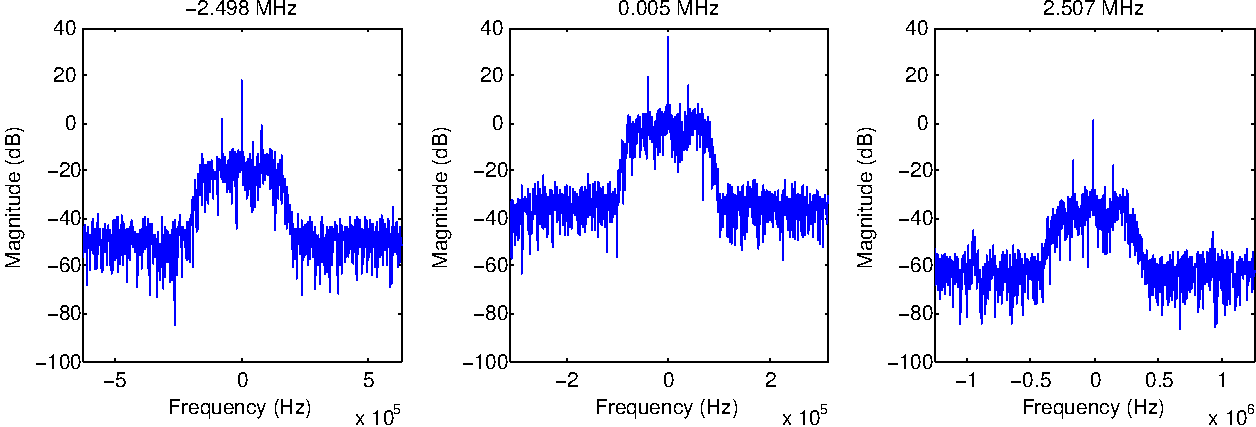
\includegraphics[width=\textwidth]{cyclo_poly_results}%
\caption{Output of the combined cyclostationary detector and polyphases channelizer. All three test signals sampled at four samples per symbol.}
\label{fig:cyclo_poly_results}
\end{figure}

Figure~\ref{fig:cyclo_poly_results} shows the output of this simulation when run
on our test signal. Note the small peaks in the $2.5$ MHz signal around $\pm1$
MHz - these are not present in the original signal, they are produced from
aliasing in the analysis channelizer, which can be seen in the corresponding
outputs in Figure~\ref{fig:polyphase_splits}.
% 0.9375 MHz, to be exact

\section{Overlap-Save Filter Bank}
\label{sec:sim_os}
The final module is the Overlap-Save Filter Bank. The Filter Bank is
implemented with tuning performed in the frequency domain by circular shifting
the FFT, as shown in Figure \ref{fig:overlap_save_shift}. The
simulation cannot be configured to tune in the time domain at this time.

The channelizer is fully implemented in \texttt{overlap\_save\_channelizer(...)}.
The function accepts three important parameters which determine how it
operates: 1) a list of center frequencies to tune, 2) a list of decimation
factors corresponding to each frequency, and 3) an FFT size.
% TODO: make this a definition list?

The first step performed in this function is determining the value of the
variable $P$. This corresponds to the length of the filter used, and determines
the amount of overlap in each FFT. $P$ must be greater than or equal to the
length of the longest filter and $P-1$ must be a factor of the FFT size.
A different filter must be generated for each unique decimation factor, and the
function assumes that the longest filter response will be for the narrowest
filter - the filter for the largest decimation factor. So in order to determine
$P$, the function first determines the length of the nyquist filter for the
largest decimation factor, then rounds up until $P-1$ is the nearest factor of
the FFT size. All the filters will be zero-padded to this length.

Next, the FFTs (overlapped by $P-1$ samples) are computed, and they are re-used
to tune, filter and decimate each channel.

TODO: discuss that filters are same as polyphase

\subsection{Adding Cyclo Detection}
\label{sec:sim_os_cyclo}
As discussed in Section \ref{sec:os_advantages} a major advantage to the
Overlap-Save Filter Bank is that the Forward FFTs can be re-used to estimate
the SCD. This is implemented in the simulation function
\texttt{cyclo\_and\_overlap\_save(...)}. This function uses two parts of the
overlap-save channelizer separately.  First it uses \texttt{os\_fft(...)} to
determine $P$ and compute overlapped FFTs, then it uses these FFTs to perform
cyclostationary detection, and finally it uses the FFTs again in the second part,
\texttt{os\_filter(...)}, to tune, filter, and decimate each detected channel.

Note that this process uses the same \texttt{cyclo\_detect(...)} function 
described in Section \ref{sec:sim_cyclo}, but it had to be modified to accept
either time-domain sampled data or frequency domain data. If it receives
time-domain data it performs an FFT to enter the frequency domain, but if it
receives frequency domain data it skips that step.

Decimation factors are determined to output a fixed number of samples per symbol.

Figure \ref{fig:cyclo_os_results} shows the output of this filter bank. In this
particular test every channel was demodulated with a 0\% Bit Error Rate.

\begin{figure}[bh!]
    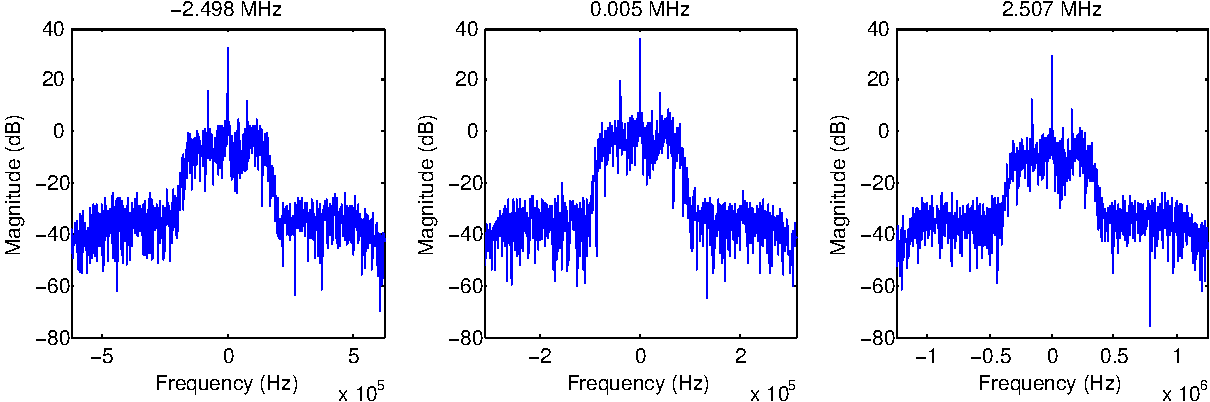
\includegraphics[width=\textwidth]{cyclo_os_results}%
\caption{Output of the combined cyclostationary detector and overlap-save filter bank. All three test signals sampled at four samples per symbol.}
\label{fig:cyclo_os_results}
\end{figure}

\chapter{Conclusion}
\label{sec:conclusion}
\markright{Brian H. Hulette \hfill Chapter \ref{sec:conclusion}. Conclusion \hfill}

% Future work
% - using single FFT to estimate cyclic spectra for non-perfect cyclic frequencies
% - fancy polyphase channelizer

%%%%%%%%%%%%%%%%%
%
% Include an EPS figure with this command:
%   \epsffile{filename.eps}
%

%%%%%%%%%%%%%%%%
%
% Do tables like this:

% \begin{table}
% \caption{The Graduate School wants captions above the tables.}
%\begin{center}
% \begin{tabular}{ccc}
% x & 1 & 2 \\ \hline
% 1 & 1 & 2 \\
% 2 & 2 & 4 \\ \hline
% \end{tabular}
%\end{center}
% \end{table}

%%%%%%%%%%%%%%%%%%%%%%%%%%%%%%%%

% If you are using BibTeX, uncomment the following:
\nocite{*}
\bibliographystyle{IEEEtran}
\bibliography{bibliography}
%
% Otherwise, uncomment the following:
% \chapter*{Bibliography}

\appendix

% In LaTeX, each appendix is a "chapter"
\chapter{Project Source}
\label{sec:source}
\markright{Brian H. Hulette \hfill Appendix \ref{sec:source}. Project Source \hfill}
% TODO: make sure this is a link - and make the project public!
The full source is hosted on GitHub
(\url{https://github.com/TheNeuralBit/cyclo\_channelizer}). Some of the
critical files are included in this appendix.

\section{Cyclostationary Detection}
\subsection{\texttt{cyclo\_detect.m}}
\lstinputlisting{../cyclo/cyclo_detect.m}
\subsection{\texttt{cyclic\_spectrum.m}}
\lstinputlisting{../cyclo/cyclic_spectrum.m}
\subsection{\texttt{single\_fft\_cyclo.m}}
\lstinputlisting{../cyclo/single_fft_cyclo.m}
\subsection{\texttt{compute\_cyclo\_fft.m}}
\lstinputlisting{../cyclo/compute_cyclo_fft.m}

\section{Polyphase Channelizer}
\subsection{\texttt{polyphase\_channelizer.m}}
\lstinputlisting{../channelize/analysis_channelizer.m}
\subsection{\texttt{analysis\_channelizer.m}}
\lstinputlisting{../channelize/analysis_channelizer.m}
\subsection{\texttt{synthesis\_channelizer.m}}
\lstinputlisting{../channelize/synthesis_channelizer.m}

\section{Overlap-Save Channelizer}
\subsection{\texttt{overlap\_save\_channelizer.m}}
\lstinputlisting{../channelize/overlap_save_channelizer.m}
\subsection{\texttt{os\_fft.m}}
\lstinputlisting{../channelize/os_fft.m}
\subsection{\texttt{os\_filter.m}}
\lstinputlisting{../channelize/os_filter.m}

\end{document}
